\chapter{Modelo de predicción}
Queremos proponer un modelo, o mejor dicho, una combinación de modelos para poder predecir cómo acabará la clasificación al final de la próxima jornada (que aún no ha comenzado a disputarse) de la Liga Española de Fútbol. Para ello tendremos que estimar el resultado más probable para cada uno de los 10 partidos que se van a disputar y calcular el nuevo ranking usando esos resultados. Tendremos que calcular tres probabilidades para cada enfrentamiento:
\begin{itemize}
	\item La probabilidad de que $a$ gane a $b$: $P(a-b=1)$.
	\item La probabilidad de que $a$ y $b$ empaten: $P(a-b=X)$.
	\item La probabilidad de que $a$ pierda ante $b$: $P(a-b=2)$.
\end{itemize}
Para estimarlas proponemos tener en cuenta lo siguiente:
\begin{itemize}
	\item La posición relativa en la tabla.
	\item La tendencia de cada equipo a lo largo de los últimos partidos.
\end{itemize}

El modelo de predicción necesita una fase inicial de ``entrenamiento'': unas primeras jornadas en las que no realizaremos predicciones sino que recogeremos datos de los resultados de los partidos disputados que luego usaremos en los distintos modelos de predicción. Comenzaremos a realizar predicciones a partir de la jornada número 21 de cada temporada, para asegurarnos que tenemos unos datos fiables que podamos usar tanto en el modelo de interpolación como en el de tendencia de los equipos. Además de que para entonces la clasificación se habrá estabilizado y no habrá cambios bruscos como los que se suelen dar al inicio de la temporada.

\section{Probabilidad basada en la posición relativa}
El valor va a depender de la diferencia entre las posiciones que ocupan los equipos en la clasificación, $r(a)-r(b)$, cuyo valor pertenece al intervalo $[-19,19] \backslash \{0\}$, dado que participan un total de 20 equipos.\\

\newpage

El primer paso es re-escalar el intervalo $[-19,19]$ en el $[0,1]$ mediante alguna función como:
\begin{center}
	$ \psi: [-19,19] \longrightarrow [0,1]$\\
	$ t \longmapsto \dfrac{t+19}{38}$
\end{center}

En los rankings con los que vamos a trabajar no se pueden producir empates, por tanto, nunca habrá dos equipos que tengan la misma posición, es decir, $r(a)-r(b)\neq 0$ y $\psi \neq \frac{1}{2}$.\\

El siguiente paso será definir unos umbrales de victoria para el equipo local, empate y victoria visitante en tres escenarios muy distintos:
\begin{itemize}
	\item El primero de la clasificación contra el último: $\psi = 0$.
	\item Equipos en posiciones consecutivas en la clasificación. \\
	Se pueden dar dos casos, que el local esté un puesto por encima del visitante en la clasificación, donde $r(a)-r(b) = -1$ y $\psi = \frac{18}{38}$, o que sea el visitante el que está un puesto por encima del local, donde $r(a)-r(b)=1$ y $\psi = \frac{20}{38}$. En adelante, al referiremos a ``equipos consecutivos'' hacemos referencia al segundo caso, es decir, cuando $\psi=\frac{20}{38}$.
	\item El último de la clasificación contra el primero: $\psi = 1$.
\end{itemize}

Gráficamente podemos resumirlo como se muestra en la figura \ref{fig:umbrales}.

\begin{figure}[H]
		\centering
		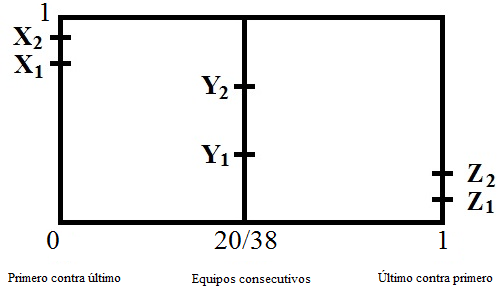
\includegraphics{images/umbrales.png}
		\caption{Umbrales de victoria local, empate y victoria visitante.} \label{fig:umbrales}
\end{figure}

Dónde los valores $X_{1},X_{2},Y_{1},Y_{2},Z_{1},Z_{2} \in [0,1]$ se identifican del siguiente modo:
\begin{itemize}
	\item Si $a$ es el primero de la clasificación y $b$ el último:\\
	 $[0,X_{1}]$ mide la probabilidad de que gane $a$, $[X_{1},X_{2}]$ mide la probabilidad de que $a$ y $b$ empaten y $[X_{2},1]$ mide la probabilidad de que gane $b$.
	 Es decir,\\
	 
	 $\begin{cases}
	 	P_{r}(a-b=1)=X_{1}\\
	 	P_{r}(a-b=X)=X_{2}-X_{1} \ \ \ \ \ \ \ \text{siendo} \ 0 \leq X_{1} \leq X_{2} \leq 1\\
	 	P_{r}(a-b=2)=1-X_{2} 
	 \end{cases}$\\
	 
	\item Análogamente, si $a$ y $b$ tienen puestos consecutivos en el ranking:\\
	
	$\begin{cases}
	P_{r}(a-b=1)=Y_{1}\\
	P_{r}(a-b=X)=Y_{2}-Y_{1} \ \ \ \ \ \ \ \text{siendo} \ 0 \leq Y_{1} \leq Y_{2} \leq 1\\
	P_{r}(a-b=2)=1-Y_{2} 
	\end{cases}$\\
	
	\item Finalmente, si $a$ es el último de la clasificación y $b$ el primero:\\
	
	$\begin{cases}
	P_{r}(a-b=1)=Z_{1}\\
	P_{r}(a-b=X)=Z_{2}-Z_{1} \ \ \ \ \ \ \ \text{siendo} \ 0 \leq Z_{1} \leq Z_{2} \leq 1\\
	P_{r}(a-b=2)=1-Z_{2} 
	\end{cases}$
\end{itemize}

Estos umbrales se obtienen de un histórico de resultados de partidos disputados. Sin embargo, es poco común que a lo largo de la temporada se enfrenten varias veces el equipo que va primero en la clasificación contra el que ocupa el último puesto, lo mismo ocurre para los enfrentamientos entre el último y el primer clasificado. En la tabla que se muestra a continuación aparece el número de partidos (con su correspondiente resultado) que se han disputado entre el líder y el colista en la última temporada, en todas las temporadas desde el año 2000 y desde 1990.

\begin{table}[H]
	\centering
	\begin{tabular}{|c|c|c|c|c|c|c|}
		\hline
		& \multicolumn{3}{|c|}{Primero vs Último} & \multicolumn{3}{|c|}{Último vs Primero} \\ \cline{2-7}
		& Gana local & Empate & Gana visit. & Gana local & Empate & Gana visit. \\ \hline 
		Solo 2014/2015 & 0 & 0 & 0 & 0 & 0 & 1 \\ \hline
		Desde 2000 & 7 & 0 & 1 & 3 & 2 & 6 \\ \hline
		Desde 1990 & 14 & 0 & 3 & 7 & 6 & 11 \\ \hline
	\end{tabular}
\end{table}

Los umbrales son imprescindibles para hacer la interpolación y obtener resultados útiles en la predicción, por lo que debemos tener suficientes observaciones para garantizarlo. Los resultados de una única temporada (la que está en juego) son totalmente inútiles ya que es probable que no se hayan enfrentado el primero contra el último en ninguna ocasión. Que se enfrenten equipos consecutivos en el ranking es algo más frecuente y con una sola temporada tendríamos observaciones suficientes para obtener unos umbrales fiables, sin embargo, no varían sustancialmente si tomamos mayores intervalos de tiempo.\\ 

Por ello, para realizar la interpolación usaremos los valores obtenidos analizando todos los resultados desde la temporada 1990/1991. La idea sería ``actualizar'' la función de interpolación recalculando los umbrales solo cuando cambiemos de temporada ya que los umbrales no suelen variar jornada a jornada.\\

Si analizamos todos los resultados desde la temporada 1990/1991 hasta la jornada actual de la temporada 2014/2015 obtendremos los siguientes porcentajes:

\begin{table}[H]
	\centering
	\begin{tabular}{|c|c|c|c|c|c|c|c|c|}
		\hline
		\multicolumn{3}{|c|}{Primero vs Último} & \multicolumn{3}{|c|}{Consecutivos} & \multicolumn{3}{|c|}{Último vs Primero} \\ \hline
		Local & Empate & Visit. & Local & Empate & Visit. & Local & Empate & Visit.\\ \hline 
		0.824 & 0 & 0.176 & 0.478 & 0.259 & 0.263 & 0.292 & 0.250 & 0.458 \\ \hline
	\end{tabular}
\end{table}

Y de la tabla anterior obtenemos los umbrales:
$$X_{1}=0.8235294117647058 \ \ \ Y_{1}=0.4782608695652174 \ \ \ Z_{1}=0.2916666666666667$$
$$X_{2}=0.8235294117647058 \ \ \ Y_{2}=0.7368421052631580 \ \ \ Z_{2}=0.5416666666666667$$

Para el resto de escenarios tenemos que interpolar de forma lineal hallando 4 rectas (las que unen $X_{1}$ a $Y_{1}$, $Y_{1}$ a $Z_{1}$, $X_{2}$ a $Y_{2}$ y $Y_{2}$ a $Z_{2}$).\\

De esta forma tenemos dos funciones $f,g:[0,1] \longrightarrow [0,1]$ que de forma genérica serán:

$f(n)= \begin{cases}
X_{2}+\dfrac{Y_{2}-X_{2}}{\frac{20}{38}}n \ \ \ \ \ \ \ \ \ \ \ \ \text{    si } n\leq \frac{20}{38} \\
Y_{2}+\dfrac{(n-\frac{20}{38})(Z_{2}-Y_{2})}{1-\frac{20}{38}} \ \ \text{    si } n > \frac{20}{38}
\end{cases}$

$g(n)= \begin{cases}
X_{1}+\dfrac{Y_{1}-X_{1}}{\frac{20}{38}}n \ \ \ \ \ \ \ \ \ \ \ \ \text{    si } n\leq \frac{20}{38} \\
Y_{1}+\dfrac{(n-\frac{20}{38})(Z_{1}-Y_{1})}{1-\frac{20}{38}} \ \ \text{    si } n > \frac{20}{38}
\end{cases}$
\ \\

Usando los umbrales que obtenemos tras analizar los resultados de la temporada 1990/1991 hasta la 2014/2015 la función de interpolación lineal es la siguiente:

\begin{figure}[H]
	\centering
	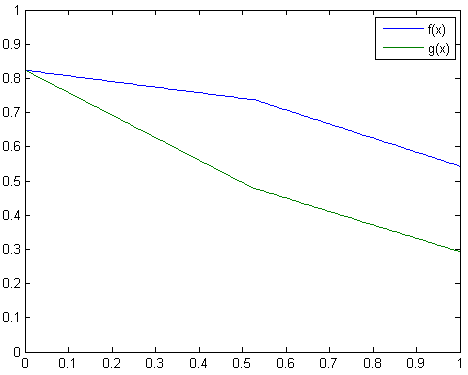
\includegraphics[scale=0.7]{images/interpolacion.png}
	\caption{Función de interpolación lineal.}
\end{figure}

También se han probado otras formas de interpolar, en concreto el uso del polinomio interpolador de Lagrange de grado 2 para obtener las funciones $f$ y $g$. Sin embargo la variación de las tres probabilidades a calcular es mínima y en ningún partido cambia el resultado final que predice la interpolación lineal. Por ello, no propondremos otros modelos de interpolación y en adelante solamente utilizaremos la interpolación lineal.  

\section{Probabilidad basada en la tendencia del equipo}
Para cada equipo trabajaremos con dos series históricas: una serie con los resultados en casa y otra serie con los resultados fuera de casa, ambos ponderados según una función memoria.\\

Para cada equipo $a$ trabajaremos con secuencias de resultados de sus últimos 5 partidos disputados como local y sus 5 últimos disputados como visitante. Almacenaremos la información cronológicamente del partido más reciente ($t=0$) al más antiguo que vamos a considerar ($t=4$). Por ejemplo:
\begin{center}
	\begin{tabular}{|c|c|c|c|c|c|}
	\hline  & t=0 & t=1 & t=2 & t=3 & t=4 \\ 
	\hline local (l)  & 1 & 1 & X & 1 & 2\\ 
	\hline visitante (v) & 2 & 2 & X & 1 & 1\\ 
	\hline 
	\end{tabular} 
\end{center}
De forma que para la jornada siguiente la probabilidad de que el equipo en cuestión gane, empate o pierda como local es:
\begin{center}
$P_{l}(a - \star=1)=\dfrac{m(0)+m(1)+m(3)}{\sum_{t=0}^{4}m(t)}$\\
$P_{l}(a - \star=X)=\dfrac{m(2)}{\sum_{t=0}^{4}m(t)}$ \ \ \ \
$P_{l}(a - \star=2)=\dfrac{m(4)}{\sum_{t=0}^{4}m(t)}$
\end{center}
donde $m(t)$ es una función memoria.\\

Análogamente se calculan las probabilidades para el siguiente partido como visitante:
\begin{center}
	$P_{v}(\star - a=1)=\dfrac{m(3)+m(4)}{\sum_{t=0}^{4}m(t)}$ \ \ \ \
	$P_{v}(\star - a=X)=\dfrac{m(2)}{\sum_{t=0}^{4}m(t)}$\\
	$P_{v}(\star - a=2)=\dfrac{m(0)+m(1)}{\sum_{t=0}^{4}m(t)}$
\end{center}

La función memoria servirá para ponderar el resultado de cada equipo en función del tiempo que haya transcurrido desde el partido en cuestión. Por ejemplo, no tiene tanto valor la victoria de hace 5 partidos como tiene la derrota del último enfrentamiento.\\

Vamos a proponer tres funciones memoria distintas y en capítulos posteriores analizaremos cuál de las tres obtiene mejores resultados. 

\newpage

\begin{itemize}
	\item Función constante: todos los resultados tienen el mismo valor. $Y=1$
	\begin{figure}[H]
		\centering
		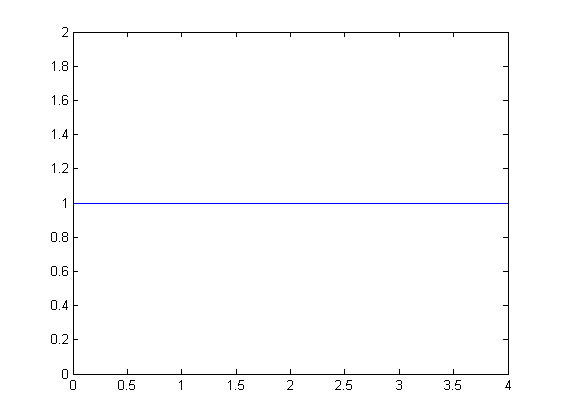
\includegraphics[scale=0.7]{images/mem1.png}
		\caption{Función memoria constante.} \label{fig:constante}
	\end{figure}
	
	\item Función lineal: $Y=5-X$
	\begin{figure}[H]
		\centering
		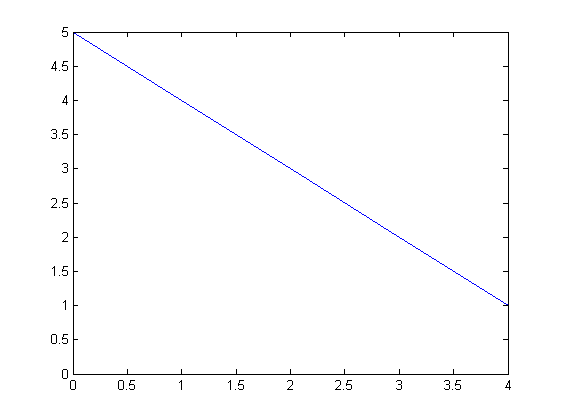
\includegraphics[scale=0.7]{images/mem2.png}
		\caption{Función memoria lineal.} \label{fig:lineal}
	\end{figure}

\newpage

	\item Función exponencial: $Y=2^{-X}$
	\begin{figure}[H]
		\centering
		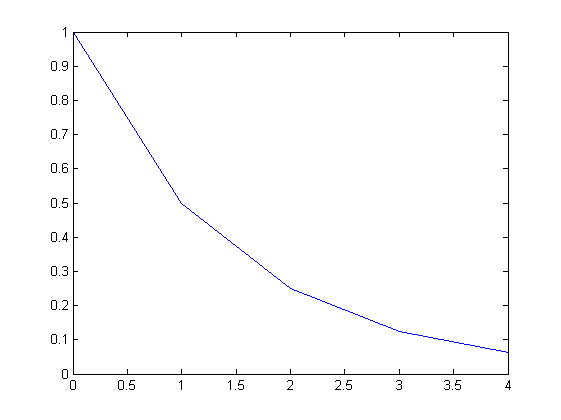
\includegraphics[scale=0.7]{images/mem3.png}
		\caption{Función memoria exponencial.} \label{fig:exponencial}
	\end{figure}	
\end{itemize}
\ \\
Para cada equipo tendremos dos probabilidades:\\
$P_{l}(a - \star=1)$, $P_{l}(a - \star=X)$ y $P_{l}(a - \star=2)$ para los partidos como local \\
$P_{v}(\star - a=1)$, $P_{v}(\star - a=X)$ y $P_{v}(\star - a=2)$ para los partidos como visitante\\

Para pronosticar el resultado del enfrentamiento $a-b$ debemos conjuntar $P_{l}(a - \star)$ con $P_{v}(\star - b)$ usando la siguiente tabla:

\begin{center}
	\begin{tabular}{|c|c|c|c|}
	\hline  & $P_{l}(a - \star=1)$ & $P_{l}(a - \star=X)$ & $P_{l}(a - \star=2)$ \\ 
	\hline $P_{v}(\star - b=1)$ & $(1,0,0)$ & $(\frac{1}{2},\frac{1}{3},\frac{1}{6})$ & $(\frac{1}{4},\frac{1}{2},\frac{1}{4})$  \\ 
	\hline $P_{v}(\star - b=X)$ & $(\frac{1}{2},\frac{1}{3},\frac{1}{6})$ & $(0,1,0)$ & $(\frac{1}{6},\frac{1}{2},\frac{1}{3})$ \\ 
	\hline $P_{v}(\star - b=2)$ & $(\frac{1}{4},\frac{1}{2},\frac{1}{4})$ & $(\frac{1}{6},\frac{1}{2},\frac{1}{3})$ & $(0,0,1)$ \\ 
	\hline 
\end{tabular} 
\end{center}

En las tuplas de números de la tabla anterior, el primer número es el que usaremos para calcular $P_{s}(a-b=1)$, el segundo para $P_{s}(a-b=X)$ y el tercero para $P_{s}(a-b=2)$, dicho número es por el que tenemos que multiplicar el producto de las entradas.\\

Por ejemplo, para calcular $P_{s}(a-b=1)$ la tabla que debemos usar es la compuesta por el primer elemento de cada tupla\\
\[
A_{1}= \left(\begin{array}{ccc}
1 & 1/2 & 1/4\\
1/2 & 0 & 1/6\\
1/4 & 1/6 & 0
\end{array} \right)
\]
de forma que
\begin{center}
	$P_{s}(a-b=1)=$\\
	$1\cdotp P_{l}(a - \star=1)P_{v}(\star - b=1) + \frac{1}{2}\cdotp P_{l}(a - \star=X)P_{v}(\star - b=1) + \frac{1}{4}\cdotp P_{l}(a - \star=2)P_{v}(\star - b=1)+$\\ 
	$\frac{1}{2}\cdotp P_{l}(a - \star=1)P_{v}(\star - b=X) + 0\cdotp P_{l}(a - \star=X)P_{v}(\star - b=X) + \frac{1}{6}\cdotp P_{l}(a - \star=2)P_{v}(\star - b=X)+$\\
	$\frac{1}{4}\cdotp P_{l}(a - \star=1)P_{v}(\star - b=2) + \frac{1}{6}\cdotp P_{l}(a - \star=X)P_{v}(\star - b=2) + 0\cdotp P_{l}(a - \star=2)P_{v}(\star - b=2)\text{ } $ 
\end{center}
\ \\	
Es decir, $P_{s}(a-b=1)= 
\langle
(P_{v}(\star - b=1),P_{v}(\star - b=X),P_{v}(\star - b=2)) A_{1}  
\left(\begin{array}{c}
P_{l}(a - \star=1)\\
P_{l}(a - \star=X)\\
P_{l}(a - \star=2)
\end{array} \right)
\rangle $\\

Aplicaremos un razonamiento análogo para calcular $P_{s}(a-b=X)$ y $P_{s}(a-b=2)$.

\section{Combinación}
Ahora contaremos con dos probabilidades: las probabilidades basadas en la posición relativa ($P_{r}(a-b=1) \ \ P_{r}(a-b=X) \ \ P_{r}(a-b=2)$) y las basadas en la serie histórica de cada equipo ($P_{s}(a-b=1) \ \ P_{s}(a-b=X) \ \ P_{s}(a-b=2)$).\\

Para conjugarlas usaremos una combinación convexa, tomamos $\lambda \in [0,1]$ y tenemos
\begin{center}
	$ P(a-b=1) = \lambda P_{r}(a-b=1) + (1-\lambda) P_{s}(a-b=1)$\\
	$ P(a-b=X) = \lambda P_{r}(a-b=X) + (1-\lambda) P_{s}(a-b=X)$\\
	$ P(a-b=2) = \lambda P_{r}(a-b=2) + (1-\lambda) P_{s}(a-b=2)$
\end{center}
Debiendo optimizar $\lambda$ para obtener el mejor resultado posible entrenándolo sobre el histórico de datos.